\documentclass[../main.tex]{subfiles}

\graphicspath{{\subfix{../imgs/}}}

\begin{document}

\section{Challenges}
\begin{frame}[c]
    \frametitle{Challenges}
    1. Separation of clustered nuclei.

    \begin{figure}
        \centering
        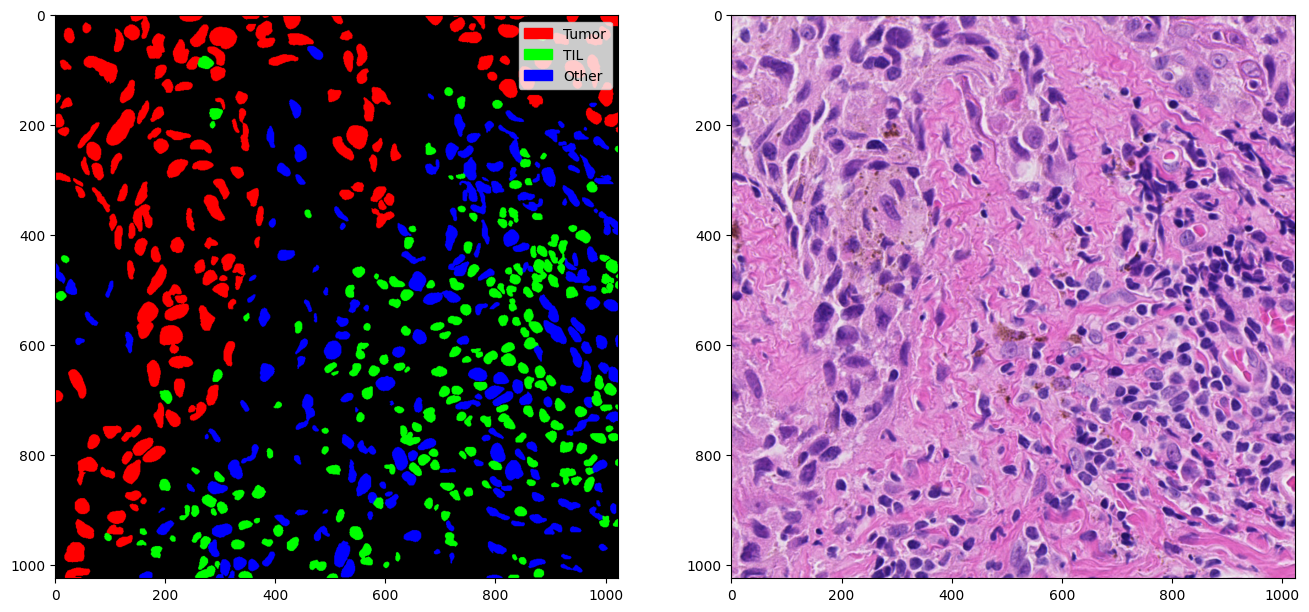
\includegraphics[width=0.8\textwidth]{example_data.png}
        \caption{Example of tumor, TIL and other nuclei.}
    \end{figure}
\end{frame}

\begin{frame}[c]
    \frametitle{Challenges}
    2. Separation of different classes of nuclei.

    \begin{figure}
        \centering
        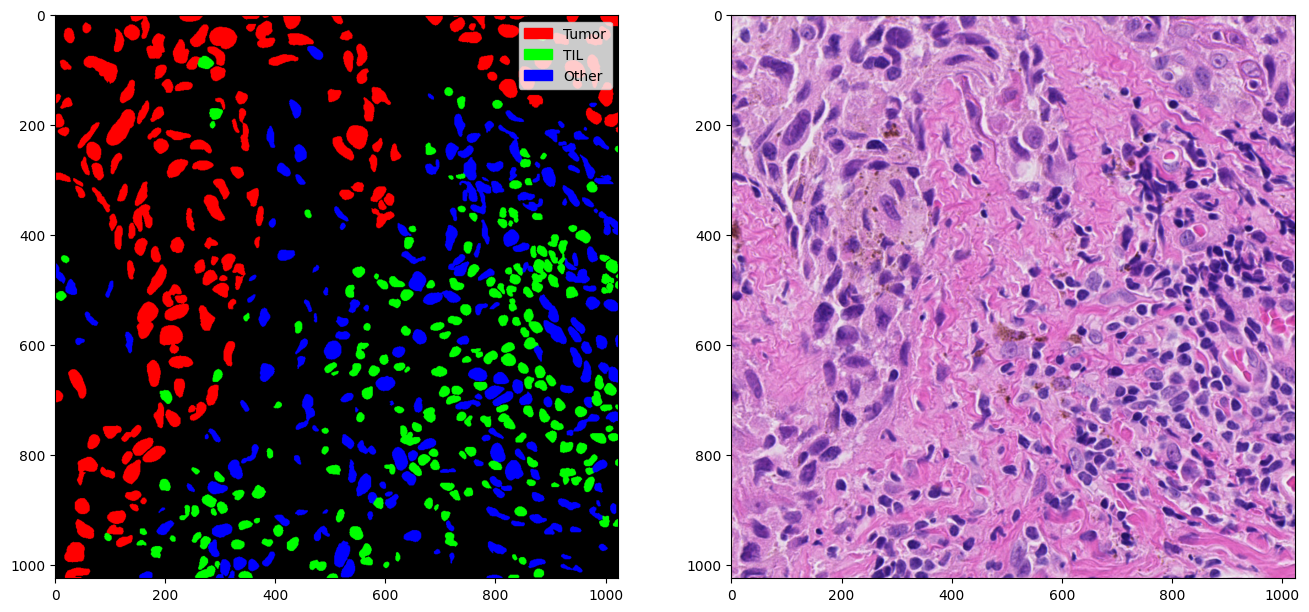
\includegraphics[width=0.8\textwidth]{example_data.png}
        \caption{Example of tumor, TIL and other nuclei.}
    \end{figure}
\end{frame}

\begin{frame}[c]
    \frametitle{Challenges}
    3. Class imbalance.

    \begin{figure}
        \centering
        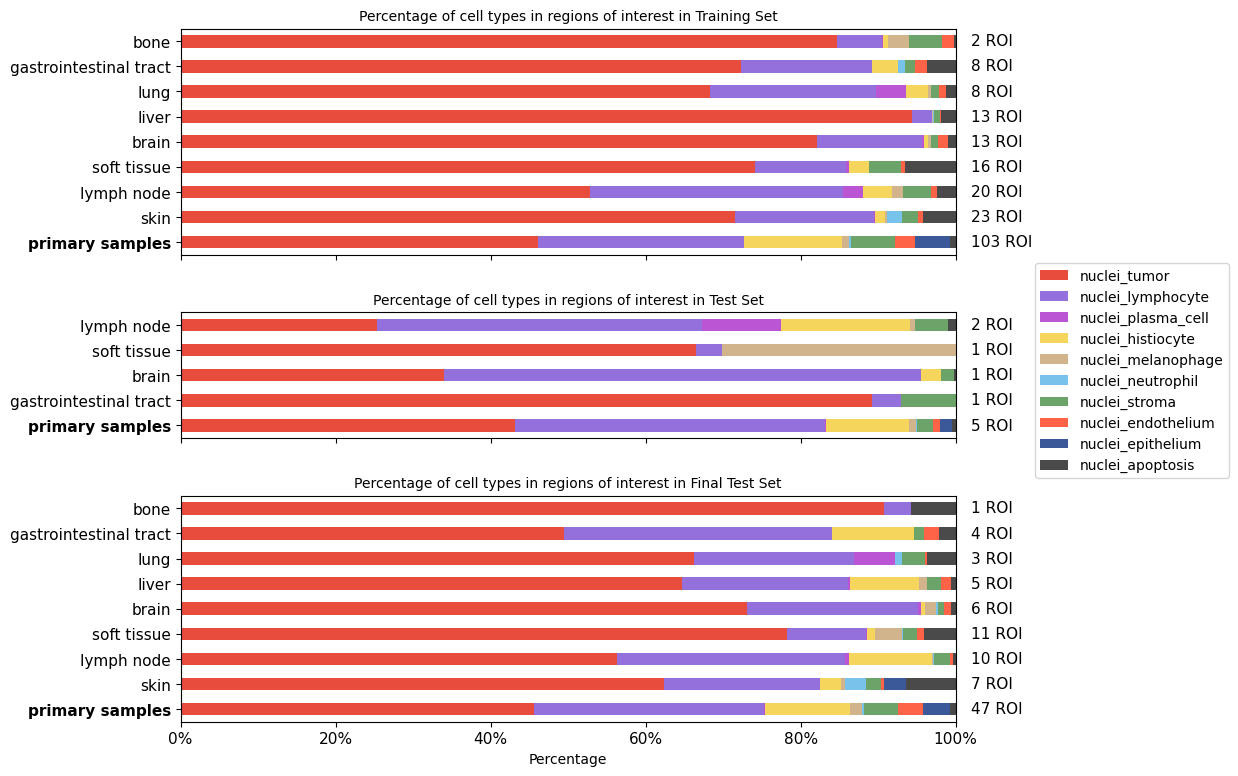
\includegraphics[width=0.8\textwidth]{nuclei_distribution.png}
        \caption{Percentage distribution of nuclei in datasets.}
    \end{figure}
\end{frame}

\begin{frame}[c]
    \frametitle{Challenges}
    4. Low performance of transfer learning.

    \begin{block}{Typical Method}
        \begin{itemize}
            \item Many older techniques rely on a HoverNet pre-trained on the PanNuke dataset.
            \item Results in suboptimal performance due to melanomas ability of mimicking other cell types.
        \end{itemize}
    \end{block}
\end{frame}

\end{document}